\chapter{Drugi rozdzia�}
Lorem ipsum dolor sit amet, consectetur adipiscing elit. Vivamus elementum arcu nec blandit aliquam. Integer eros dolor, molestie eget dictum quis, luctus sit amet sapien. Proin dignissim felis in ornare volutpat. Morbi vulputate rutrum efficitur. Ut vehicula vehicula metus, et iaculis tortor mattis vel. Nam blandit, arcu quis ultricies blandit, libero ante commodo augue, in accumsan dui leo at orci. Phasellus in augue et velit pulvinar malesuada ut et sem. Nulla vehicula nibh eu odio sollicitudin sagittis. Praesent condimentum semper neque, tincidunt luctus nisl scelerisque sed. Orci varius natoque penatibus et magnis dis parturient montes, nascetur ridiculus mus.

Donec in libero a enim tempor finibus. Etiam in turpis sed metus ultricies pharetra vitae a ipsum. Nullam elementum est a vehicula convallis. Praesent vel eleifend quam, id eleifend tortor. Vestibulum non sollicitudin arcu. Nunc ultricies, ex sit amet faucibus elementum, erat est finibus lacus, non porttitor metus mi sed purus. Mauris at volutpat quam. Nam vel varius elit. Donec a urna vitae felis posuere facilisis. Suspendisse id enim quis massa imperdiet ultrices quis eu nibh. Pellentesque in elit ut tortor pharetra condimentum. Fusce non dapibus arcu, non blandit odio. Suspendisse faucibus fermentum neque quis dapibus.
\section{Pierwsza sekcja}
Maecenas tincidunt est sit amet porttitor suscipit. Nullam rutrum lectus ut odio cursus facilisis. Donec fermentum, dolor sed sagittis congue, augue nisi sagittis nulla, nec ultricies sem elit non nibh. Vivamus erat ante, volutpat nec lectus in, finibus iaculis velit. Phasellus vel hendrerit dolor. Cras gravida ac lacus sit amet euismod. Integer venenatis ut tortor id tristique. Lorem ipsum dolor sit amet, consectetur adipiscing elit. Curabitur pellentesque ut ex ac volutpat. Suspendisse pellentesque tempus tempus. Nullam pharetra purus nunc, vitae eleifend ligula consectetur vel. Mauris quis quam non massa vestibulum lobortis. Donec suscipit tortor ut dictum vestibulum. Vestibulum ante ipsum primis in faucibus orci luctus et ultrices posuere cubilia Curae; Praesent ut finibus risus. Suspendisse sed risus ultricies, accumsan metus vitae, dignissim justo.
\subsection{Pierwsza podsekcja}

\begin{figure}[ht]
\centering
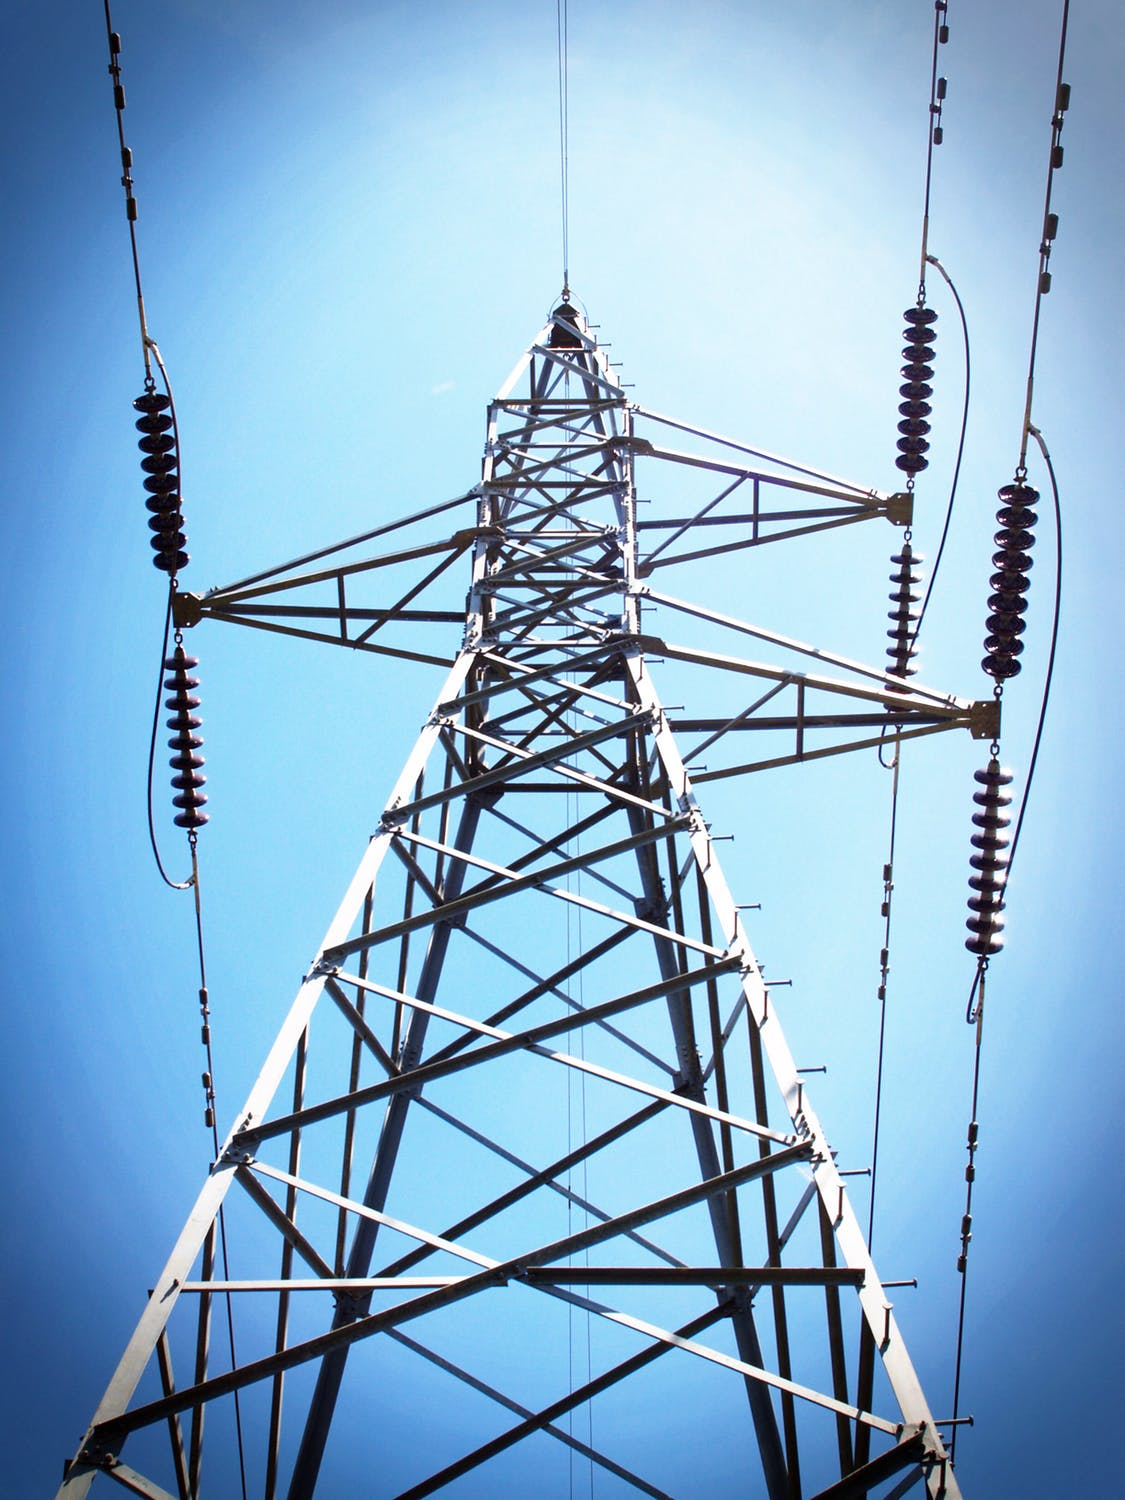
\includegraphics[scale=0.25]{rysunki/example}
\caption{Przyk�adowy obraz zamieszczony w pracy dyplomowej}
\label{img/template1}
\end{figure}
Vestibulum lorem elit, ornare vitae ultrices non, rhoncus eu elit. Vestibulum et gravida erat. Sed ut velit sollicitudin, blandit libero nec, maximus felis. Morbi feugiat pharetra lacus sit amet sodales. Aenean a sem elit. Ut et augue justo. Sed id consequat magna, non tincidunt eros. Sed congue tellus vitae ipsum commodo, nec pretium quam congue. Fusce non imperdiet sem, at imperdiet nibh. Morbi convallis nisl ante. Maecenas hendrerit, augue ac pretium molestie, ex massa lacinia est, sit amet volutpat eros magna vel erat.

Nunc egestas mauris sit amet sem facilisis, in rutrum quam faucibus. Etiam ornare fringilla tellus, sit amet bibendum nulla fermentum vitae. Nullam nec consectetur ipsum. Duis pulvinar libero vel diam lacinia, ac dapibus massa malesuada. Nullam sit amet gravida risus, nec tincidunt enim. Integer vehicula, nisl vitae hendrerit molestie, arcu arcu eleifend enim, at tempus odio leo nec nibh. Sed ut tortor risus. Nulla mattis pretium gravida. Phasellus eu augue magna. Proin quis dolor consectetur, accumsan velit et, maximus ipsum. 

Vestibulum lorem elit, ornare vitae ultrices non, rhoncus eu elit. Vestibulum et gravida erat. Sed ut velit sollicitudin, blandit libero nec, maximus felis. Morbi feugiat pharetra lacus sit amet sodales. Aenean a sem elit. Ut et augue justo. Sed id consequat magna, non tincidunt eros. Sed congue tellus vitae ipsum commodo, nec pretium quam congue. Fusce non imperdiet sem, at imperdiet nibh. Morbi convallis nisl ante. Maecenas hendrerit, augue ac pretium molestie, ex massa lacinia est, sit amet volutpat eros magna vel erat.

\begin{table}[ht]
\captionsetup{justification=centering}
\caption{Dane techniczne silnika nap�dowego uk�adu jezdnego}
\centering
    \begin{tabular}{|l|l|c|}
    \hline
    \multicolumn{1}{|l|}{\textbf{Lp.}} & \multicolumn{1}{l|}{\textbf{Parametr}} & \multicolumn{1}{c|}{\textbf{Warto��}} \\
    \hline
       1.   & Napi�cie zasilania [V] & 12  \\
    \hline
       2.   &  Pr�dko�� obrotowa [obr/min]& 200\\
    \hline
       3.  & Moment obrotowy [Nm]   & 0.8 \\
    \hline
       4.  & Maks. pr�d pracy [A]      &  0.8 \\
    \hline
       5.  & �rednica wa�u [mm]     &  8 \\
    \hline
       6.  & Rodzaj czujnika     &  Inkrementalny   \\
    \hline
       7.  & Rozdzielczo�� enkodera [imp/obr]   &  75 \\
    \hline
    \end{tabular}
  \label{silnik_skret}
\end{table}

Nunc egestas mauris sit amet sem facilisis, in rutrum quam faucibus. Etiam ornare fringilla tellus, sit amet bibendum nulla fermentum vitae. Nullam nec consectetur ipsum. Duis pulvinar libero vel diam lacinia, ac dapibus massa malesuada. Nullam sit amet gravida risus, nec tincidunt enim. Integer vehicula, nisl vitae hendrerit molestie, arcu arcu eleifend enim, at tempus odio leo nec nibh. Sed ut tortor risus. Nulla mattis pretium gravida. Phasellus eu augue magna. Proin quis dolor consectetur, accumsan velit et, maximus ipsum. 



Nunc egestas mauris sit amet sem facilisis, in rutrum quam faucibus. Etiam ornare fringilla tellus, sit amet bibendum nulla fermentum vitae. Nullam nec consectetur ipsum. Duis pulvinar libero vel diam lacinia, ac dapibus massa malesuada. Nullam sit amet gravida risus, nec tincidunt enim. Integer vehicula, nisl vitae hendrerit molestie, arcu arcu eleifend enim, at tempus odio leo nec nibh. Sed ut tortor risus. Nulla mattis pretium gravida. Phasellus eu augue magna. Proin quis dolor consectetur, accumsan velit et, maximus ipsum. 


Nunc egestas mauris sit amet sem facilisis, in rutrum quam faucibus. Etiam ornare fringilla tellus, sit amet bibendum nulla fermentum vitae. Nullam nec consectetur ipsum. Duis pulvinar libero vel diam lacinia, ac dapibus massa malesuada. Nullam sit amet gravida risus, nec tincidunt enim. Integer vehicula, nisl vitae hendrerit molestie, arcu arcu eleifend enim, at tempus odio leo nec nibh. Sed ut tortor risus. Nulla mattis pretium gravida. Phasellus eu augue magna. Proin quis dolor consectetur, accumsan velit et, maximus ipsum. 

\begin{equation}
\label{rownanie}
\sum_{n=1}^{\infty} 2^{-n} \arccos(\frac{\int_{a}^{b} x^2 dx}{x})  = 1
\end{equation}

Nunc egestas mauris sit amet sem facilisis, in rutrum quam faucibus. Etiam ornare fringilla tellus, sit amet bibendum nulla fermentum vitae. Nullam nec consectetur ipsum. Duis pulvinar libero vel diam lacinia, ac dapibus massa malesuada. Nullam sit amet gravida risus, nec tincidunt enim. Integer vehicula, nisl vitae hendrerit molestie, arcu arcu eleifend enim, at tempus odio leo nec nibh. Sed ut tortor risus. Nulla mattis pretium gravida. Phasellus eu augue magna. Proin quis dolor consectetur, accumsan velit et, maximus ipsum. 

\lstset{style=matlab}

\begin{lstlisting}[caption={Przyk�adowy listing programu Matlab}]
for n = 1 : 4
    
    for j = 1 : 100
        Imp_1_100(n,j) = (R1*R2*C2*i*j*2*pi + R1 + R2);
    end
    
    % Zmiana warto�ci  
    
    if log(abs(Imp_1_100(n,100))) - log(Rr) <= 2
        Rr = Rr/10;
    end
    
    RT(n) = Rr;  % Przypisanie warto�ci
end
\end{lstlisting}


\lstset{style=java}

\begin{lstlisting}[caption={Przyk�adowy listing w j�zyku Java},label=javovy]
class OuterClass {
  int x = 10;

  private class InnerClass {
    int y = 5;
  }
}

public class MyMainClass {
  public static void main(String[] args) {
    OuterClass myOuter = new OuterClass();
    OuterClass.InnerClass myInner = myOuter.new InnerClass();
    System.out.println(myInner.y + myOuter.x);
  }
}
\end{lstlisting}

\newpage





\lstset{style=vhdl}

\begin{lstlisting}[caption={Przyk�adowy listing w j�zyku VHDL}]

architecture FSMD of gcd is
begin

    process(rst, clk)

    -- define states using variable 
    type S_Type is (ST0, ST1, ST2);
    variable State: S_Type := ST0 ;			
    variable Data_X, Data_Y: unsigned(3 downto 0);
	
    begin

        if (rst='1') then		    -- initialization
	    d_o <= "0000";
	    State := ST0;
	elsif (clk'event and clk='1') then
	    case State is
	        when ST0 =>		    -- starting
		    if (go_i='1') then
			Data_X := x_i;
			Data_Y := y_i;
			State := ST1;
		    else
		        State := ST0;
		    end if;
		when ST1 =>		    -- idle state 
		    State := ST2;
		when ST2 =>		    -- computation
		    if (Data_X/=Data_Y) then
		        if (Data_X<Data_Y) then
			    Data_Y := Data_Y - Data_X;
			else
			    Data_X := Data_X - Data_Y;
			end if;
			State := ST1;
		    else
			d_o <=Data_X;       -- done
		        State := ST0;
		    end if;
		when others =>		    -- go back 
		    d_o <= "ZZZZ";
		    State := ST0;
            end case;				
 	end if;
    
    end process;		

end FSMD;

\end{lstlisting}


Nunc egestas mauris sit amet sem facilisis, in rutrum quam faucibus. Etiam ornare fringilla tellus, sit amet bibendum nulla fermentum vitae. Nullam nec consectetur ipsum. Duis pulvinar libero vel diam lacinia, ac dapibus massa malesuada. Nullam sit amet gravida risus, nec tincidunt enim. Integer vehicula, nisl vitae hendrerit molestie, arcu arcu eleifend enim, at tempus odio leo nec nibh. Sed ut tortor risus. Nulla mattis pretium gravida. Phasellus eu augue magna. Proin quis dolor consectetur, accumsan velit et, maximus ipsum. 
Nunc egestas mauris sit amet sem facilisis, in rutrum quam faucibus. Etiam ornare fringilla tellus, sit amet bibendum nulla fermentum vitae. Nullam nec consectetur ipsum. Duis pulvinar libero vel diam lacinia, ac dapibus massa malesuada. Nullam sit amet gravida risus, nec tincidunt enim. Integer vehicula, nisl vitae hendrerit molestie, arcu arcu eleifend enim, at tempus odio leo nec nibh. Sed ut tortor risus. Nulla mattis pretium gravida. Phasellus eu augue magna. Proin quis dolor consectetur, accumsan velit et, maximus ipsum. 

Nunc egestas mauris sit amet sem facilisis, in rutrum quam faucibus. Etiam ornare fringilla tellus, sit amet bibendum nulla fermentum vitae. Nullam nec consectetur ipsum. Duis pulvinar libero vel diam lacinia, ac dapibus massa malesuada. Nullam sit amet gravida risus, nec tincidunt enim. Integer vehicula, nisl vitae hendrerit molestie, arcu arcu eleifend enim, at tempus odio leo nec nibh. Sed ut tortor risus. Nulla mattis pretium gravida. Phasellus eu augue magna. Proin quis dolor consectetur, accumsan velit et, maximus ipsum. 



% Definition of blocks:
\tikzset{%
  block/.style    = {draw, thick, rectangle, minimum height = 3em,
    minimum width = 3em},
  sum/.style      = {draw, circle, node distance = 2cm}, % Adder
  input/.style    = {coordinate}, % Input
  output/.style   = {coordinate} % Output
}
% Defining string as labels of certain blocks.
\newcommand{\suma}{\Large$+$}
\newcommand{\inte}{$\displaystyle \int$}
\newcommand{\derv}{\huge$\frac{d}{dt}$}

\begin{figure}[ht]

\begin{tikzpicture}[auto, thick, node distance=2cm, >=triangle 45]
\draw
	% Drawing the blocks of first filter :
	node at (0,0)[right=-3mm]{\Large }
	node [input, name=input1] {} 
	node [sum, right of=input1] (suma1) {\suma}
	node [block, right of=suma1] (inte1) {\inte}
         node at (6.8,0)[block] (Q1) {\Large $Q_1$}
         node [block, below of=inte1] (ret1) {\Large$T_1$$$};
    % Joining blocks. 
    % Commands \draw with options like [->] must be written individually
	\draw[->](input1) -- node {$X(Z)$}(suma1);
 	\draw[->](suma1) -- node {} (inte1);
	\draw[->](inte1) -- node {} (Q1);
	\draw[->](ret1) -| node[near end]{} (suma1);
	% Adder
\draw
	node at (5.4,-4) [sum, name=suma2] {\suma}
    	% Second stage of filter 
	node at  (1,-6) [sum, name=suma3] {\suma}
	node [block, right of=suma3] (inte2) {\inte}
	node [sum, right of=inte2] (suma4) {\suma}
	node [block, right of=suma4] (inte3) {\inte}
	node [block, right of=inte3] (Q2) {\Large$Q_2$$$}
	node at (9,-8) [block, name=ret2] {\Large$T_2$$$}
;
	% Joining the blocks of second filter
	\draw[->] (suma3) -- node {} (inte2);
	\draw[->] (inte2) -- node {} (suma4);
	\draw[->] (suma4) -- node {} (inte3);
	\draw[->] (inte3) -- node {} (Q2);
	\draw[->] (ret2) -| (suma3);
	\draw[->] (ret2) -| (suma4);
         % Third stage of filter:
	% Defining nodes:
\draw
	node at (11.5, 0) [sum, name=suma5]{\suma}
	node [output, right of=suma5]{}
	node [block, below of=suma5] (deriv1){\derv}
	node [output, right of=suma5] (sal2){}
;
	% Joining the blocks:
	\draw[->] (suma2) -| node {}(suma3);
	\draw[->] (Q1) -- (8,0) |- node {}(ret1);
	\draw[->] (8,0) |- (suma2);
	\draw[->] (5.4,0) -- (suma2);
	\draw[->] (Q1) -- node {}(suma5);
	\draw[->] (deriv1) -- node {}(suma5);
	\draw[->] (Q2) -| node {}(deriv1);
    	\draw[<->] (ret2) -| node {}(deriv1);
    	\draw[->] (suma5) -- node {$Y(Z)$}(sal2);
    	% Drawing nodes with \textbullet
\draw
	node at (8,0) {\textbullet} 
	node at (8,-2){\textbullet}
	node at (5.4,0){\textbullet}
    	node at (5,-8){\textbullet}
    	node at (11.5,-6){\textbullet}
    	;
	% Boxing and labelling noise shapers
	\draw [color=gray,thick](-0.5,-3) rectangle (9,1);
	\node at (-0.5,1) [above=5mm, right=0mm] {\textsc{generator szumu I rz�du}};
	\draw [color=gray,thick](-0.5,-9) rectangle (12.5,-5);
	\node at (-0.5,-9) [below=5mm, right=0mm] {\textsc{generator szumu II rz�du}};
\end{tikzpicture}
\caption{Przyk�adowy schemat blokowy utworzony przy u�yciu pakietu tikz}
\end{figure}

Nunc egestas mauris sit amet sem facilisis, in rutrum quam faucibus. Etiam ornare fringilla tellus, sit amet bibendum nulla fermentum vitae. Nullam nec consectetur ipsum. Duis pulvinar libero vel diam lacinia, ac dapibus massa nc egestas mauris sit amet sem facilisis, in rutrum quam faucibus. Etiam ornare fringilla tellus, sit amet bibendum nulla fermentum vitae. Nullam nec consectetur ipsum. Duis pulvinar libero vel diam lacinia, ac dapibus massa.



